\setlength{\footskip}{8mm}

\chapter{Methodology}
\label{ch:methodology}

\textit{The different components of the system and how they work together are described in this chapter.}

\section{Hardware}

In the current system, the Mobius Maxi action cam, with a fish-eye lens is mounted on a rigid base. The PixHawk 2.4.8 flight controller, having an IMU and a GPS module, is attached to the same rigid base. 


The data from both devices are fed into a computer with an i7 CPU and 16 GB of RAM running Ubuntu 16.04. The PixHawk 2.4.8 has PX4 as its firmware. Both the PixHawk and camera are connected to the computer through the USB interface. In the Mobius camera's settings, autofocus and auto white balance are turned off. 

The test rig is shown in Figure \ref{fig:rigsetup}. The test rig is mounted on top of radio controlled vehicle, the Tamiya Bullhead. 

\begin{figure}[htp]
	
	\centering
	\subfloat[]{%
	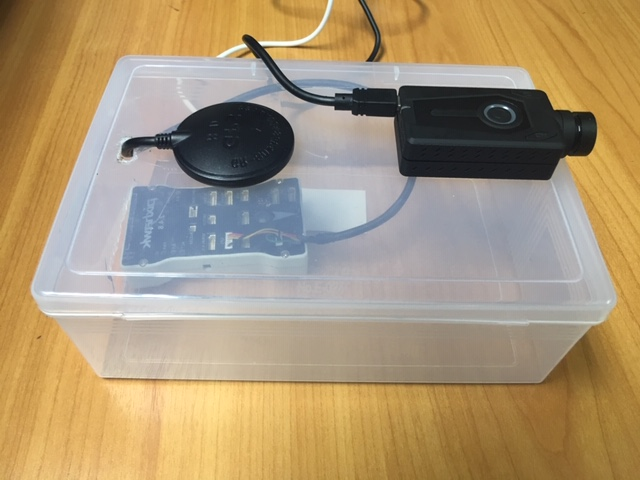
\includegraphics[width=.3\textwidth]{figures/rig}%
	}
	\subfloat[]{%
	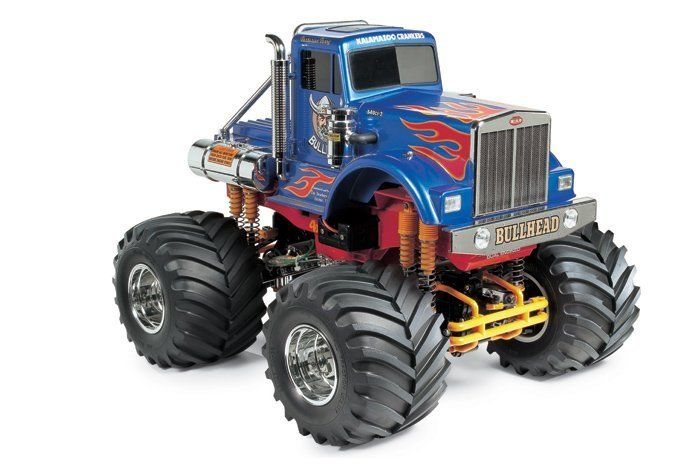
\includegraphics[width=.3\textwidth]{figures/tamiya_bullhead}
	}
	\subfloat[]{%
	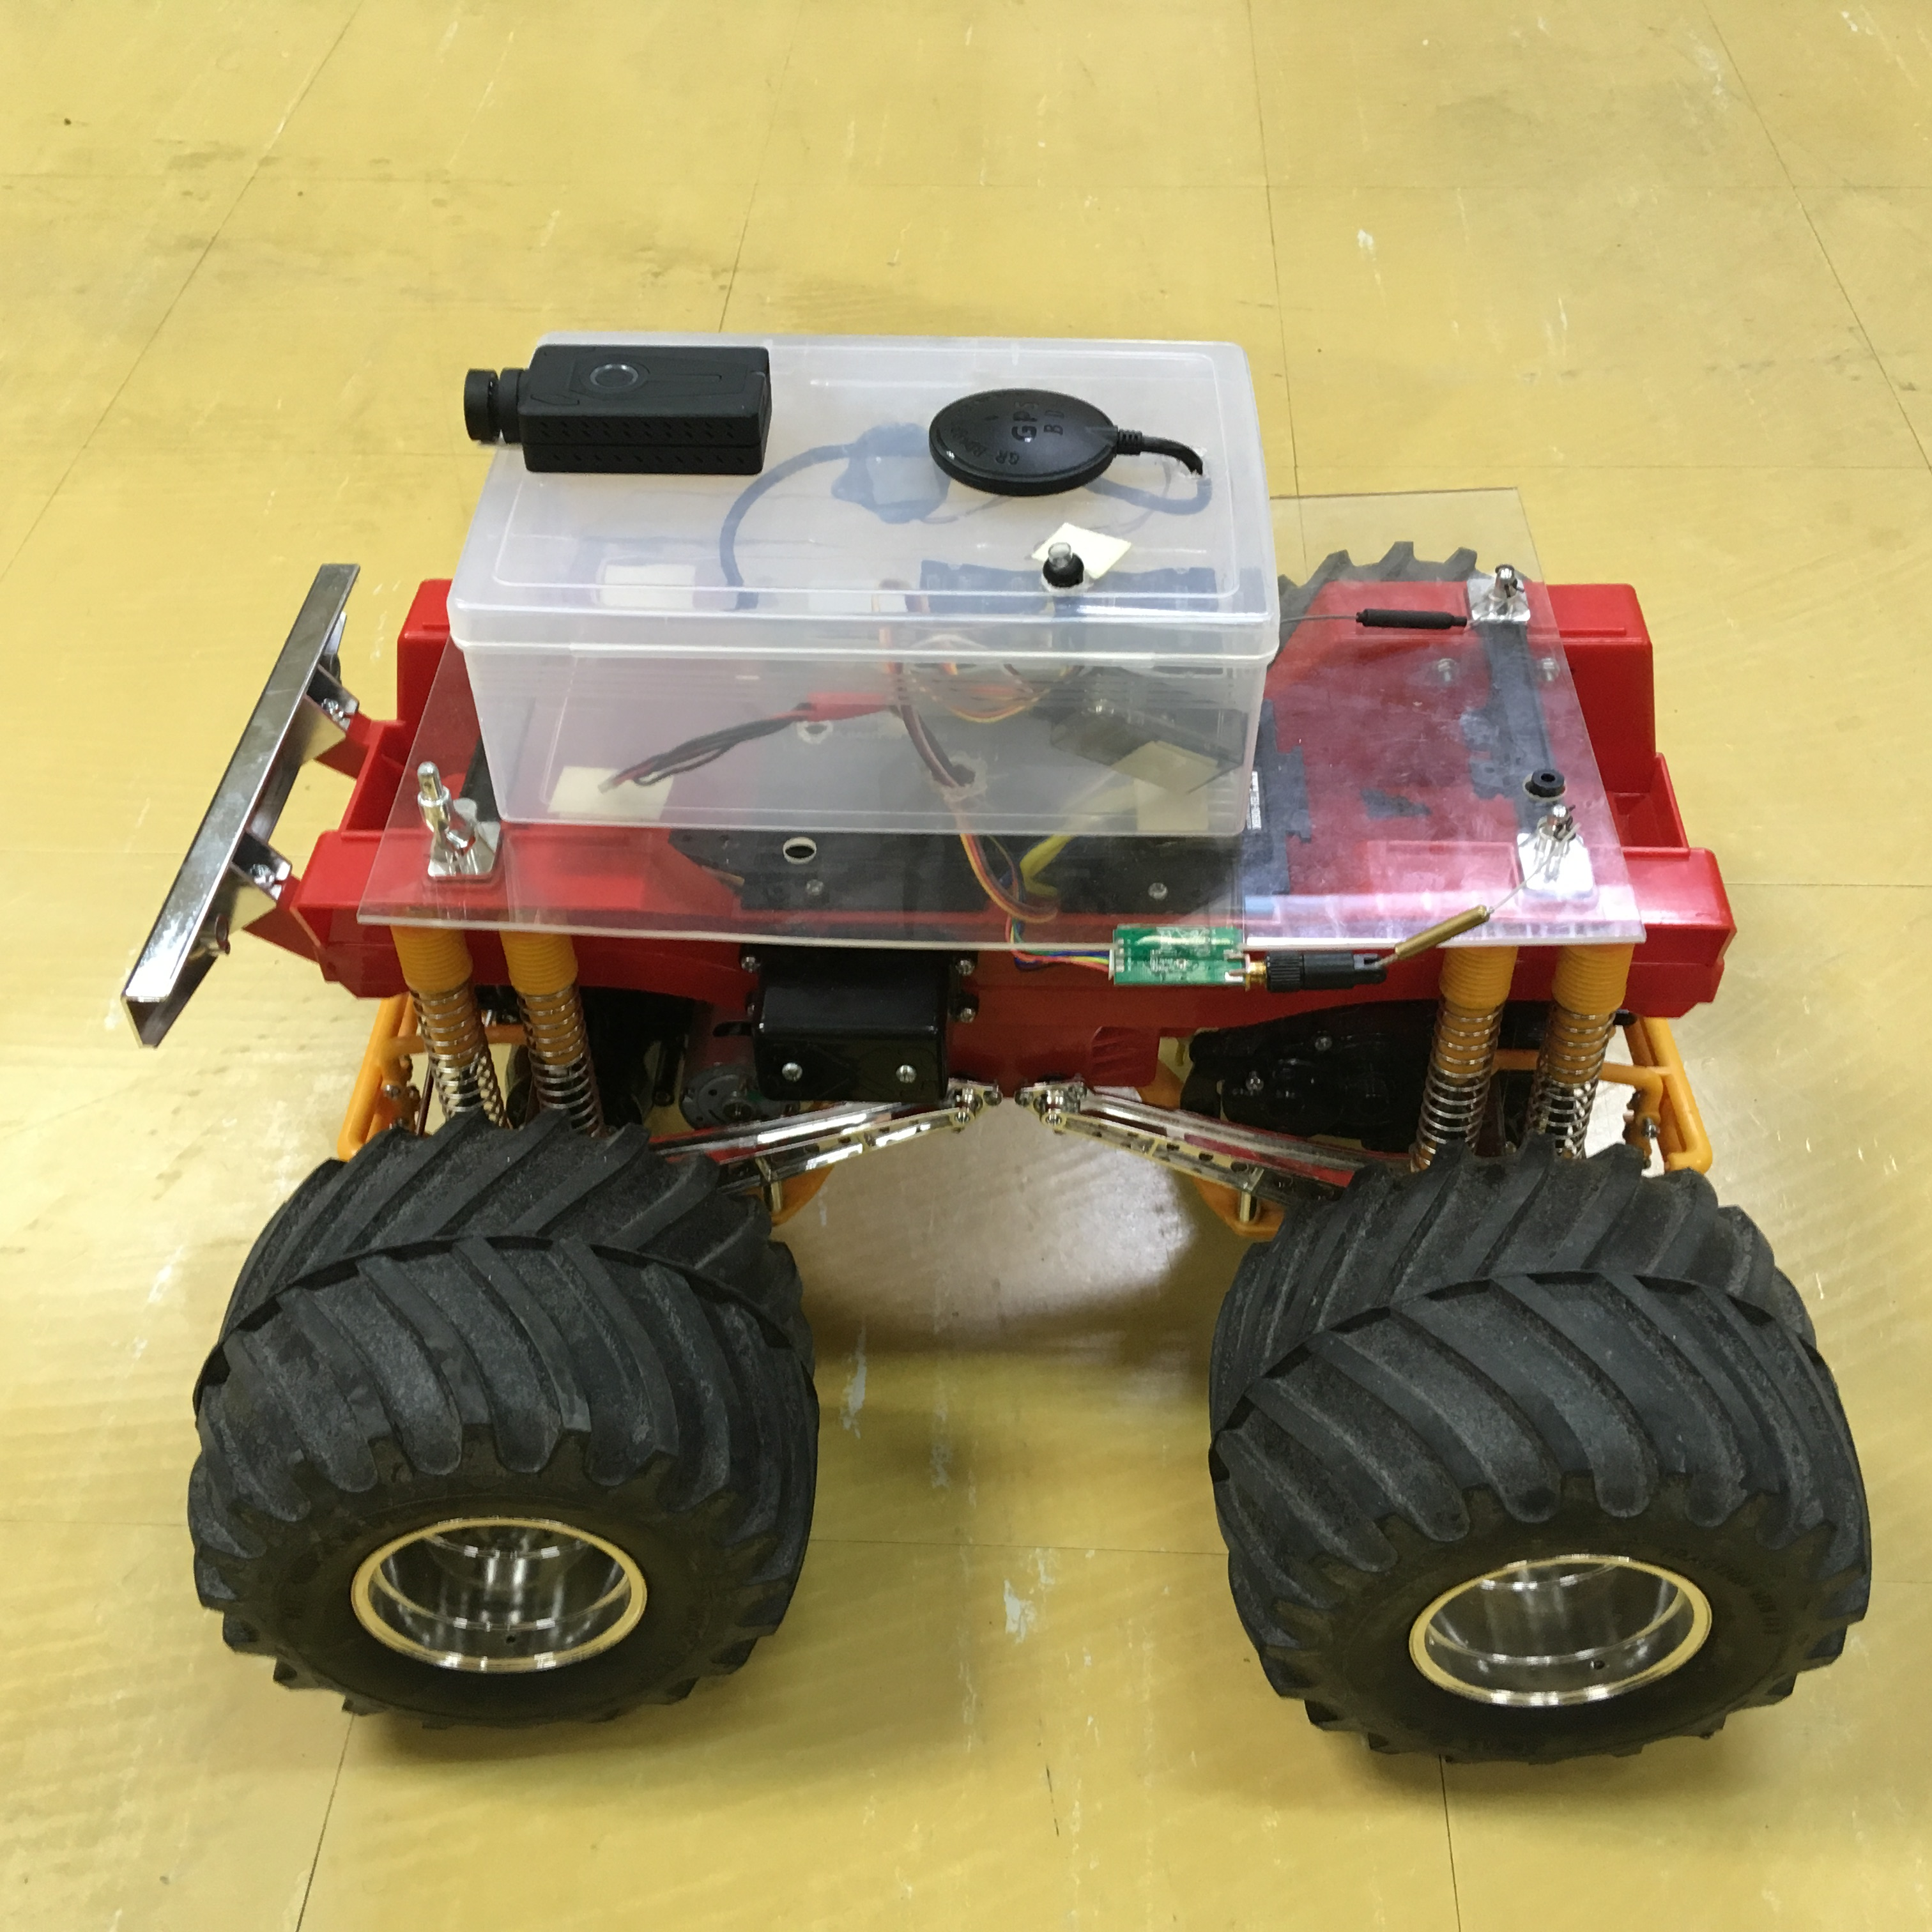
\includegraphics[width=.3\textwidth]{figures/rover-rig}
	}
	\caption[Test platform.]{\small 
		Test Platform. (a) Close up of the test setup. (b) Tamiya Bullhead. (c) Test rig mounted on top of the Tamiya Bullhead.}
	\label{fig:rigsetup}
	
\end{figure}


\section{Software}
The Robot Operating System (ROS) version Kinetic is running on the test laptop. 
The software components on the test laptop are as follows and shown in Figure~\ref{fig:rosgraph}.

\begin{figure} \label{fig:rosgraph}
	\centering
	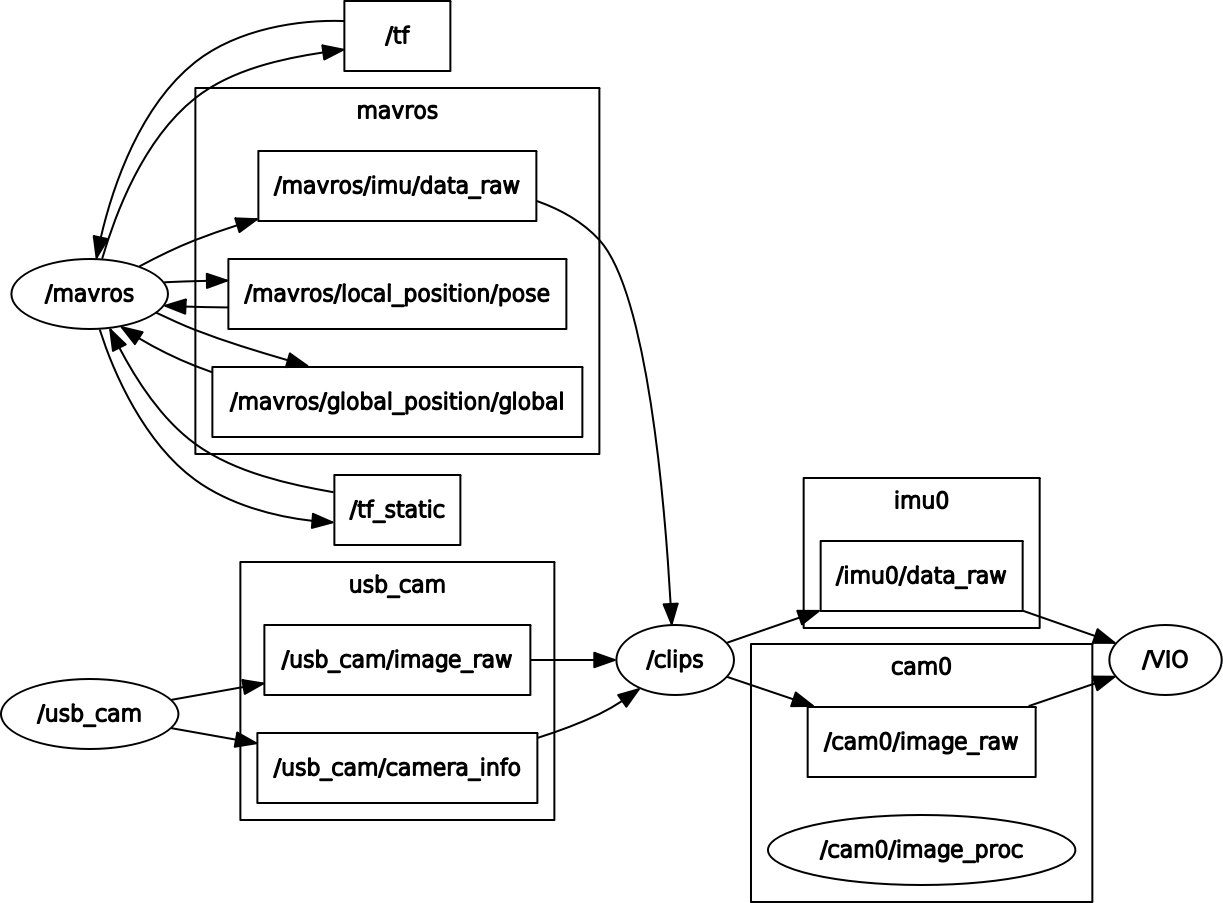
\includegraphics[width=5in]{figures/rosgraph}
	\caption[ROS node tunning on test machine]{\small 
		ROS nodes running on test machine. }
\end{figure}

\begin{itemize}
	\item usb\_cam: Modified to support H264 streams.
	\item mavros: Communicates with PixHawk using the MAVLINK protocol.
	\item clips: A new middleware layer I created to ensure there is at least one IMU report message between each pair of image frames.
	\item LearnVIORB: Modified to publish pose, point clouds, and tf information.
\end{itemize}

\subsection{usb\_cam node}
The Mobius Maxi supports H264 hardware encoding. The video stream captured through this H264 stream is smoother and supports higher framerates than the raw stream. The usb\_cam package directly captures the video stream from USB cam, but it does not support H264 streams.
The library \textit{libavutils} used by the package does however support H264 streams. I added support for the \textit{h264} pixel format parameter and a new color format parameter that can accept either \textit{yuv422p} or \textit{yuv420p} to make the package stream the H264 video feed from Mobius Maxi to the other ROS components.
 
\subsection{mavros}
The test machine runs mavros to communicate with PixHawk flight controller. 
The PixHawk connection is shown as serial port \texttt{/dev/ttyACM0} on the test computer. The baud rate is chosen as \textit{921600}.
PX4 publishes coordinates using the NED convention. Mavros automatically converts the NED coordinates to ENU coordinates to use with ROS.

Time synchronization between PX4 and ROS is automatically done by the \textit{sys\_time} mavros plugin.
A timesync message $M$ is sent at a consistent frequency from the host system to FCU. The host system timestamps the message with the current time $t_s$. The remote system then receives it and adds its timestamp $t_c$ to $M$ before replying back.
The offset between the host system and the remote system is calculated assuming round trip time for the message is equal in both ways.

\begin{equation}
t_{offset} = t_s + t_{now} - 2t_c
\end{equation}

The calculated $t_{offset}$ is used for interpolating the time offset and time skew. $n$ observations of $t_{offset}$ is used to converge the interpolation. $k = \{0 ... n-1\}$ is the index of the current timesync message being received for interpolation.

\begin{equation}
I = k/n
\end{equation}

$I$, the progress of the current interpolation is used in the sigmoid function given in \ref{eq:sigmoidtimesync}.

\begin{equation} \label{eq:sigmoidtimesync}
P = 1 - e^{\frac{1}{2} (1 - \frac{1}{(1 - I)})}
\end{equation}

The two coefficients, $\alpha$ and $\beta$ are calculated using \ref{eq:sigmoidalpha} and \ref{eq:sigmoidbeta}. $\alpha_i$ and $\beta_i$ are the initial constraint constants. $\alpha_f$ and $\beta_f$ are the final constraint constants.

\begin{equation} \label{eq:sigmoidalpha}
\alpha = P  \alpha_f + (1 - P)  \alpha_i
\end{equation}

\begin{equation} \label{eq:sigmoidbeta}
\beta = P  \beta_f + (1 - P)  \beta_i
\end{equation}

The interpolated time offset $t$ and time skew $t_{skew}$ is updated for each timesync messaged received until the interpolation has not converged using online exponential smoothing filter given in \ref{eq:onlinesmoothingoffset} and \ref{eq:onlinesmoothingskew}.

\begin{equation} \label{eq:onlinesmoothingoffset}
t_{k} = \alpha  t_{offset}  + (1 - \alpha)  (t_{k-1} + t_{skew_{k-1}})
\end{equation}

\begin{equation} \label{eq:onlinesmoothingskew}
t_{skew_k} = \beta  (t_k - t_{k-1}) + (1 - \beta)  t_{skew_{k-1}} 
\end{equation}

After the estimate has converged, it is used until a maximum number of consecutive observations are received that is higher than a threshold deviation from the present estimate. In this case, the estimate is re-calculated with $n$ new observations.

If the interpolation has not converged yet, the intermediate time offset and time skew values are used.


\subsection{clips}
The IMU and camera are independently connected to the test computer. They are not tightly bound. Although mavros does time synchronization, at least one IMU measurement between any two consecutive image frames is necessary for VIORB to predict the next keyframe location. 
I created clips as a middleware ROS package to ensure that there is at least one IMU measurement between two image frames. If two consecutive images are received without any IMU measurements in between, then the image frame is dropped.

\subsection{LearnVIORB}
LearnVIORB \cite{learnviorb} is a community-developed implementation of Visual Inertial ORB SLAM \shortcite{DBLP:journals/corr/Mur-ArtalT16}. This package does not publish pose and point cloud in real time. I added support for publishing pose, point cloud, and tf information as ROS topics as part of this special study. 
I referred to the open source project ORB\_SLAM2\_CUDA \cite{orbcuda}, an enhancement of ORB2 SLAM, which does publish these topics for implementation.

\subsection{PX4 firmware}
One of the requirements of VIORB is that the IMU measurements should be frequent, in the hundreds of Hz range. PX4 does not by default support more than 50 Hz. Consequently, to increase it to 200 Hz, I edited \texttt{ROMFS/px4fmu\_common/init.d/rcS} file in the source code and recompiled the firmware.
The \texttt{rcS} file is executed during each bootup.

The Ardupilot framework was an alternative to PX4, but it lacks support for 200 Hz rates.

The edit to \texttt{ROMFS/px4fmu\_common/init.d/rcS} is as follows.

\begin{verbatim}
	mavlink stream -d /dev/ttyACM0 -s ATTITUDE -r 200        
	mavlink stream -d /dev/ttyACM0 -s HIGHRES_IMU -r 200
\end{verbatim}

\section{Calibration}
For a visual inertial SLAM system to work, the camera's intrinsic parameters, the IMU noise analysis, and the camera-to-IMU transformation need to be calibrated beforehand. I provide some details here.
 
\subsection{Camera intrinsic parameters}
The camera intrinsic parameters were calibrated with the ROS \textit{camera\_calibration} package. This package uses a checkerboard pattern to calculate $K$ and the distortion parameters.

\subsection{IMU noise analysis} \label{section:imu_bias_calculation}
Stationary IMU data were recorded for a few hours. Using the \textit{kalibr\_allan} package, I calculated the noise density, and random walk parameters for the accelerometer and gyroscope using the \textit{Allan variance} method. 

\subsection{Camera-to-IMU tranformation}
VIORB requires ${\bf T}_{CB}$, the camera to IMU transformation. I used the  \textit{kalibr} tool to find the transformation matrices ${\bf T}_{CB}$ and ${\bf T}_{BC}$, where $C$ is the camera's reference frame and $B$ is the IMU's reference frame. Kalibr uses apriltags or a checkerboard pattern for calibration along with the previously described IMU noise analysis results. 

\section{Integration}
One of the requirements of VIORB SLAM is configuring the input \texttt{yaml} configuration file, which has camera IMU transformation ${\bf T}_{CB}$, camera intrinsic parameters $K$, distortion parameters, ORB feature detector settings, IMU initialization time, and camera and IMU drift time offset. The \texttt{yaml} file was created using the results of the above sections.

The IMU noise density and random walk constants in \texttt{src/IMU/imudata.cpp} was updated with the results of IMU noise analysis.


A single launch file in clips package starts usb\_cam, mavros, and clips. It publishes \texttt{/imu0/data\_raw} and \texttt{/cam0/image\_raw}. 

\begin{verbatim}
<launch>
  <node name="usb_cam" pkg="usb_cam"
     type="usb_cam_node" output="screen">
    <param name="video_device" value="/dev/video1" />
    <param name="image_width" value="640" />
    <param name="image_height" value="480" />
    <param name="framerate" value="60" />
    <param name="pixel_format" value="h264" />
    <param name="color_format" value="yuv420p" />
    <param name="camera_frame_id" value="usb_cam" />
    <param name="io_method" value="mmap"/>
  </node>
  <include file="$(find mavros)/launch/px4.launch" />
  <node name="clips" pkg="clips"
     type="clips_node" respawn="false" output="screen"/>
  <group ns="cam0">
    <node name="image_proc" pkg="image_proc"
       type="image_proc" respawn="false" output="screen"/>                       
  </group>
<launch>
\end{verbatim}

The \texttt{/imu0/data\_raw} and \texttt{/cam0/image\_raw} topics can either be directly subscribed by VIORB or it can be stored in a bag file. 

VIORB is launched using another launch file.
\begin{figure}
	\centering
	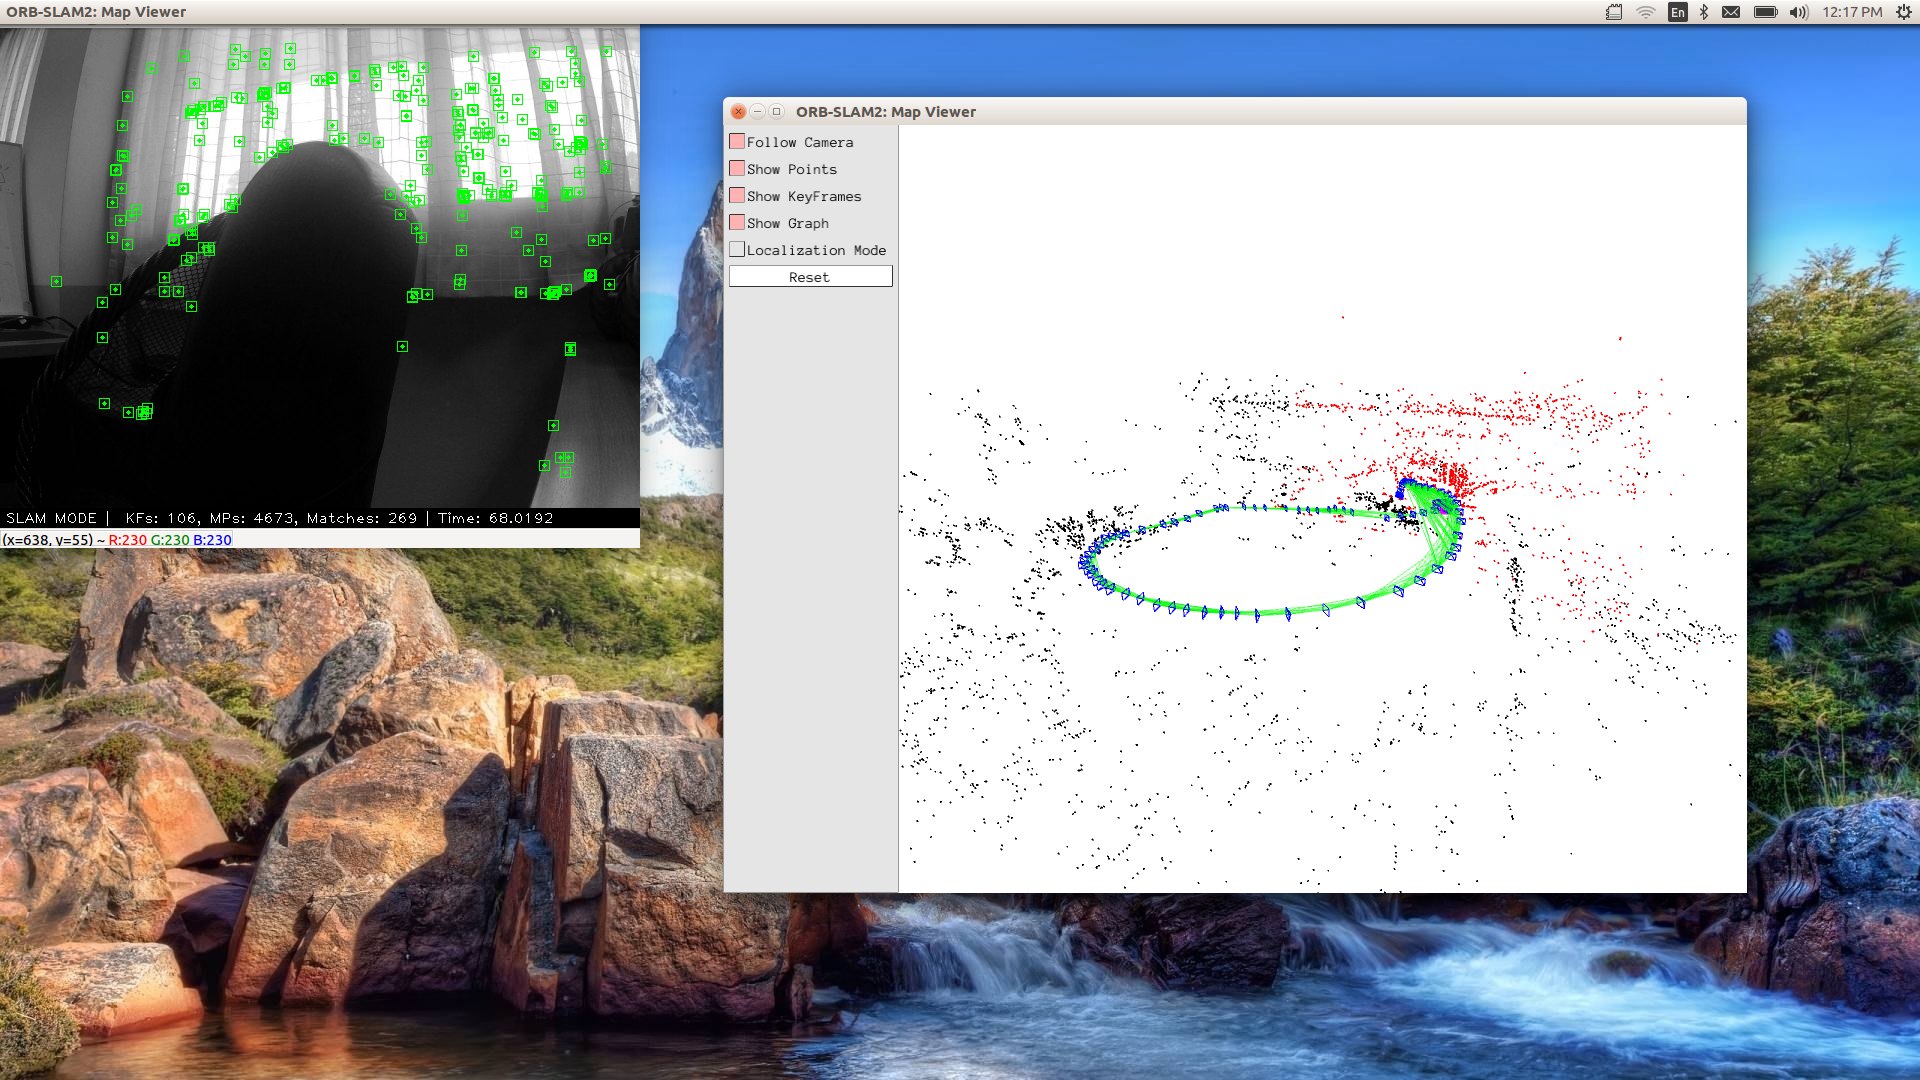
\includegraphics[width=5in]{figures/cloudpoint}
	\caption[Trial run]{\small 
		 A trial run which generates point cloud and pose in CS 203. }
\end{figure}

\FloatBarrier
